\section{Analysis}

The process of creation of CERED is mostly an attempt to execute the first two part of a pipeline we mention in the first chapter. To the best of our knowledge, there is no suitable entity linking tool for Czech. There are tools for Named Entity Recognition that we could theoretically use to our advantage if we decided to focus on named entity only.

Therefore we need to find a way, to get to similar results as the pipeline would get. We do not expect that our CERED generator will be as powerful as respective dedicated tools would be. We will not try to create a general entity recognition and linking tools - on the contrary we will exploit any extra information that chosen Wikimedia projects provide. 

There are several aspect that we need to think through. 
\begin{itemize}
  \item  Dataflow - jaké info kde vezmeme a s čím ho v jakém pořadí spojíme?
  \item  Entity Matching - jak matchoat?
  \item  Silver data - konečně přejmenovat btw! Snad čisčí?
  \item  Vztahy - jak matchovat, jaké kategorie?
  \item  zobrazovátko?
\end{itemize}



\begin{figure}[h]\centering
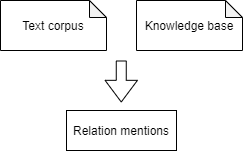
\includegraphics[width=70mm]{./img//Diplomka diagramy-Distant supervision}
\caption{Distant supervision diagram}
\label{obr03:Nhust}
\end{figure}

\subsection{Dataflow}

We are starting with two files. One being a Czech Wikipedia dump: it is a collection of articles. Each article has, among other information, its title, id and text. The other is a Wikidata dump. The simpliest way of processing those files would be to process them separately and thus obtaining sentences on one side and relations (a relation type with two items) on the other, see \ref{obr02:AVerySimple}. This approach comes with a clear disadvantage. We would lose any additional information to the sentences, that could be potentially useful (for example article title might be helpful to determine which items are mentioned in a sentence). To solve this we could precompute something for each article and attach it to each sentence, risking a massive increase in required capacity to work with such data. On a similar note, if we were to follow the diagram exactly, we would probably store item names (labels and aliases) in each relation, worsening the situation even further.

\begin{figure}
\centering
\subfloat[Uninformed approach]{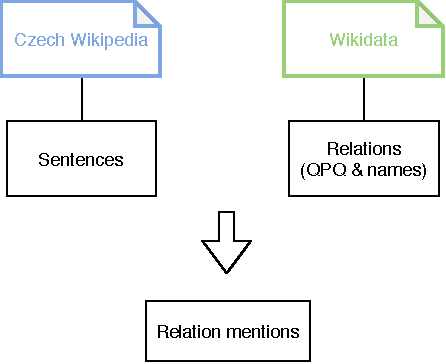
\includegraphics[width=0.4\textwidth]{./img/Diplomka diagramy-uninformed}}
\qquad
\subfloat[Informed approach]{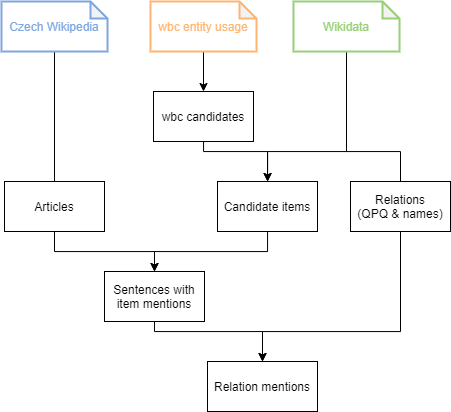
\includegraphics[width=0.6\textwidth]{./img/Diplomka diagramy-informed}}
\end{figure}

%\begin{figure}
%\centering
%\subfigure{
%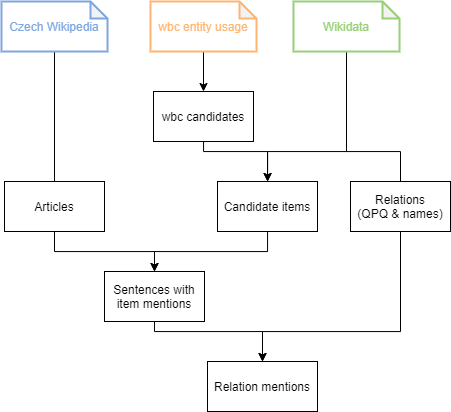
\includegraphics[width=140mm, height=117mm]{./img/Diplomka diagramy-informed}
%\caption{Zjednodušený diagram výroby korpusu}
%\label{obr03:Nhust}
%}
%\subfigure{
%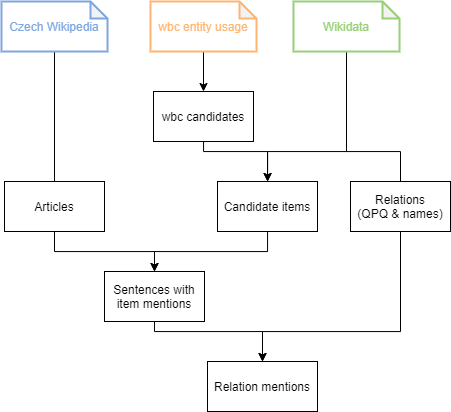
\includegraphics[width=140mm, height=117mm]{./img/Diplomka diagramy-informed}
%\caption{Zjednodušený diagram výroby korpusu}
%\label{obr03:Nhust}
%}
%%\end{figure}

We decided to update the dataflow to address those issues. We will preprocess Wikidata dump to contain only the data we will use. An item will be kept only if it has a Czech name and we will significantly reduce its statements: we will keep title of its Czech Wikipedia article and create a list of (QID,PID,QID) triples - \defineterm{QPQ}, representing statements that contained information about relations between between this and other items. This way, we have all the necessary information - article title to be able to connect article to item, names for each item to be able to find mentions of items and finally QPQ triples to connect relations and sentences.

One approach to finding item mentions in text could be called uninformed. We could assume that any item can be mentioned in any sentence. This approach seems to have two main issues: the computation would likely take quite some time but mainly we expect a huge amount of ambiguous mentions. An example of this ambiguity, that we seen as problematic might be children named after their parents. In this case, not only that the entity might get confused, moreover, if we then assign the relation, we might easily confuse a sentence mentioning a spouse relation for a parent relation mention.

On the other side, we can use the extra information that Wikimedia projects provide and opt for a more informed approach. The topic of most Czech Wikipedia articles is a Wikidata item, therefore this item is nearly certainly mentioned in the article. Some Wikidata statements were based on relevant articles and thus it seem rational to expect items, that are related to the main item of an article, to be mentioned. We decided to look only for a tiny subset of all Wikidata items in each article - \defineterm{candidate items}. As we just discussed, if an article is based on a item, than this item and all items, that are connected to it by a statement, are considered candidate items.

Czech Wikipedia maintains a wbc entity usage table, which contains information about which article uses which item. If we use this table, we are able to obtain a list of items, that should be mentioned in an article, lets call this list a \defineterm{wbc candidates}. A wbc candidate is at the same time a candidate item.

We might consider adding even a second level of relatives (items related to items that are related to the main item) but the branching factor might be relatively high and cause unwanted ambiguity. Consider an instance item like a concrete country, all countries would be second level relatives and thus a candidate item. Since countries tend to be of certain type (kingdom, republic, state etc.) there might be simply the type or some other more general name amongst their names (\todo{typografie}Q30 United States of America are also known as America or United States) and more countries might share this name.

So far we mostly discussed advantages of proposed informed approach, mainly a hope for higher precision specifically higher precision for item mentions. We should elaborate on some disadvantages as well. We are not trying to fully do entity linking. In the end, we will only use item mentions, if there are two of them in one sentence and if a QPQ that connects them exists. It is debatable whether we need an informed approach to increase relation mention precision, the necessity and improbability that this condition will be fulfilled for false positive item mentions might in fact be sufficient. 

One more way to locate item mentions are \defineterm{wikilinks}. A wikilink links a page to another page within same-language Wikipedia. First additional information this brings is simply the item mention (if the linked page or article has its main item). We can also consider the textual part of the link to be another name for the linked item. The quality and suitability of this name is to be examined and if we will find these names useful, they can be added to official Wikidata names.



sice by šlo neparalelně, ale co rychlost?

Mluvit o tom, proč nejdřív najdeme, co v článku hledat, pak to nasekáme na věty, pak matchujeme. Zmínit, kolik je jiných možností, že teoreticky by šlo ještě před rozsekáním na věty dělat entity linking ...

Detailně popsat, co kdy kam poteče + diagram


\subsection{Entity matching}

We have text on one side, gathered candidate items on the other and the goal is to label words that represent those items - entity mentions. There is a wide spectrum of complexity we might aim for, but once again, we are not trying to create a tool for entity recognition and linking. We will describe some of those complexity tears, but before that we should address some basic text manipulation that all of the matching methods will benefit from.



\defineterm{String equality}. Definitely the easiest method which just test whether 
\defineterm{String similarity}
\defineterm{Morphological analysis}
\defineterm{zájmena a více vět a tak}

 but the choice of final method was mostly based on performance measured once the implementation was done. 



Napsat, že v aj dělají často jen exact modulo zkratky a malé přípony, což tady nejde.

Ukázat nápady se sebráním linků z wikipedie a zavrhnout to

připomenout, jak moc se dá čeština skloňovat
říct, že nemá nejspíš smysl snažit se najít jen validní tvary, protože stejně v textu nejspíš nebudou nevalidní

asi mluvit o word order? a možná i implementovat

Říct, že jako kontrolní dataset budou přímo z linků

\subsection{silver data}
Co to je
proč je nejspíš větší šance na kvalitu
možná i ručně udělat měření kvality na těhle datech v druhé části


\subsection{Distant supervision assumption}
aneb jak matchovat vztahy

\subsection{možná to bude chtít zobrazovátko? aneb jak hodnotit kvalitu?}
možná navrhout nějaké random dotazy na odhalení nevalidních dat?


\subsection{Jaké kategorie?}



\begin{figure}[h]
\begin{center}
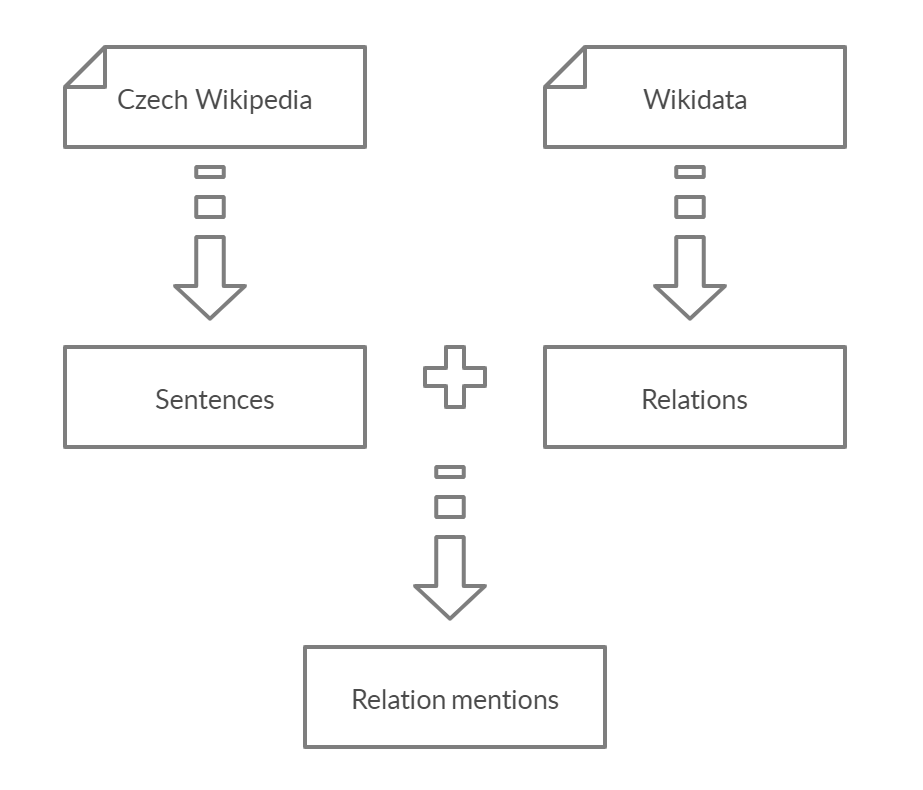
\includegraphics[width=70mm, height=60mm]{./img/a_very_simple_diagram}
\caption{A very simple diagram of dataset generation.}
\label{obr02:AVerySimple}
\end{center}
\end{figure}


\begin{figure}[p]\centering
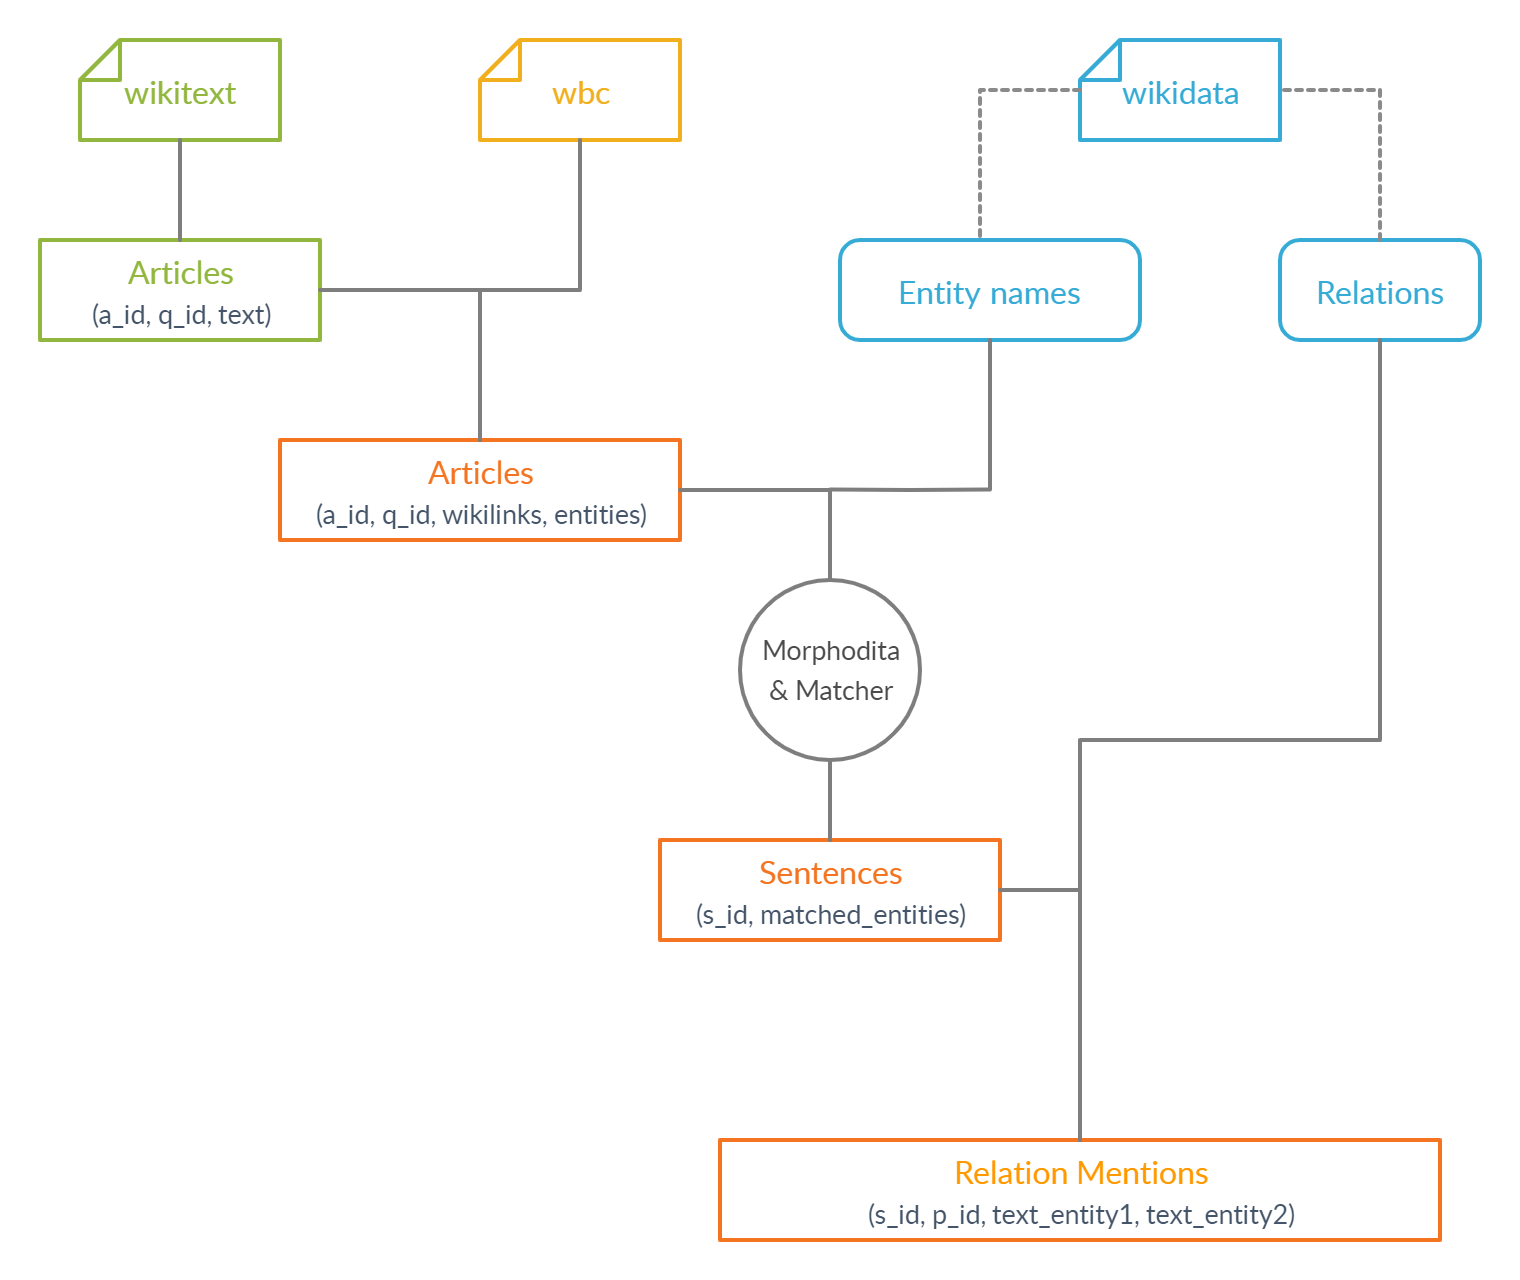
\includegraphics[width=140mm, height=117mm]{./img/Corpus_diagram}
\caption{Zjednodušený diagram výroby korpusu}
\label{obr03:Nhust}
\end{figure}